%! TEX program = pdflatex

\documentclass[oneside,solution]{karazin-prob-theory-assign}

\usepackage[utf8]{inputenc}
\usepackage[english,ukrainian]{babel}

\title{Контрольна робота}
\author{Захаров Дмитро}
\studentID{МП-31}
\instructor{Півень О.Л.}
\date{\today}
\duedate{16:00 20 березня}
\assignno{1}
\semester{Весняний семестр 2024}
\mainproblem{Варіант 5}

\begin{document}

\maketitle

% \startsolution[print]

\problem{Номер 1}

\textbf{Умова.} У кімнаті $10$ осіб, кожна з яких має номер від $1$ до $10$. Навмання вибираються 3 особи. Знайти ймовірність, що людина з більшим номером має номер $6$.

\textbf{Розв'язання.} 

Введемо ймовірнісний простір. Нехай елементарна подія -- це трійка $(n_1,n_2,n_3)$, де $n_1,n_2,n_3$ попарно різні та $n_1,n_2,n_3 \in \{1,\dots,10\}$. Відповідна універсальна множина $\Omega$ має вигляд:
\begin{equation}
    \Omega = \{(n_1,n_2,n_3) \in \{1,\dots,10\}^3: n_1 \neq n_2 \wedge n_2 \neq n_3 \wedge n_1 \neq n_3\}
\end{equation}

Нехай $A$ -- шукана подія, тобто
\begin{equation}
    A = \{(n_1,n_2,n_3) \in \Omega: \max\{n_1,n_2,n_3\} = 6\}.
\end{equation}

Скористаємось \textit{класичним визначенням ймовірності}, тобто ймовірність події $A$ знайдемо як:
\begin{equation}
    \text{Pr}[A] \triangleq \frac{|A|}{|\Omega|}
\end{equation}

Отже, залишилось порахувати кількість елементів множин $A,\Omega$. Почнемо з $\Omega$. Уявімо $3$ клітинки, на які ми ставимо числа від $1$ до $10$. На першу клітинку можемо поставити одне з $10$ значень, на друге вже $9$ (оскільки перше вже зайнято), а далі вже $8$. Тому $|\Omega| = 10 \cdot 9 \cdot 8 = 720$. 

Тепер подивимось на $A$. Нехай перша клітинка ($n_1$) зайнята числом $6$, тобто $n_1=6$. На позиції $n_2,n_3$ потрібно знайти кількість способів поставити числа \textbf{до} 6, оскільки інакше $\max\{n_1,n_2,n_3\} > 6$. Оскільки залишається 5 чисел від $1$ до $5$, то в якості $n_2$ можемо поставити $5$ чисел, а на третю клітинку $n_3$ лише $4$ числа. Тобто кількість способів дорівнює $5 \times 4 = 20$. Але! Ми врахували лише випадок $n_1=6$. Аналогічно, якщо поставити $n_2=6$ або $n_3=6$, то кількість способів так само $20$ (при цьому елементи між випадками $n_i=6$ не будуть повторюватись). Отже загальна кількість елементів $|A|=3\times 20=60$. Отже, шукана ймовірність:
\begin{equation}
    \text{Pr}[A] = \frac{60}{720} = \boxed{\frac{1}{12}}
\end{equation}

\textbf{Відповідь.} $\frac{1}{12}$.

\textit{Коментар.} При розв'язанні ми вважали, що трійки упорядковані, тобто наприклад $(n_1,n_2,n_3)$ та $(n_2,n_1,n_3)$ є різними варіантами. Якщо враховувати, що ці варіанти однакові, то $|\Omega|=C_{10}^3=120$, а $|A|=C_5^2 = 10$, звідки отримуємо ту саму ймовірність $\text{Pr}[A] = \frac{1}{12}$. Отже, в цій задачі не важлива різниця між тим, чи вважати трійки упорядкованими чи ні. 

\problem{Номер 2}

\textbf{Умова.} Три студенти складають іспит. Імовірність того, що перший студент складе іспит, дорівнює $0.95$, другий -- $0.9$, третій -- $0.85$. Визначити ймовірність того, що тільки два студенти складуть іспит.

\textbf{Розв'язання.} Нехай подія $A_i, i \in \{1,2,3\}$ полягає в тому, що $i$ студент склав іспит. Логічно вважати ці події незалежними, причому за умовою
\begin{equation}
    \text{Pr}[A_1] = 0.95, \; \text{Pr}[A_2] = 0.90, \; \text{Pr}[A_3] = 0.85.
\end{equation}

Запишемо подію $E$ -- тільки два студенти складають іспит. На мові множин, таку подію можна записати наступним чином:
\begin{equation}
    E = (\overline{A}_1 \cap A_2 \cap A_3) \cup (A_1 \cap \overline{A}_2 \cap A_3) \cup (A_1 \cap A_2 \cap \overline{A}_3),
\end{equation}
тобто або скали тільки студенти $2$ та $3$ (відповідно, при цьому студент $1$ \textbf{не} склав), або склали тільки студенти $1$ і $3$, або тільки $1$ та $2$. Наша задача тепер -- знайти $\text{Pr}[E]$, що і буде відповіддю на поставлене питання. 

По-перше помітимо, що події $\overline{A}_1 \cap A_2 \cap A_3$, $A_1 \cap \overline{A}_2 \cap A_3$ та $A_1 \cap A_2 \cap \overline{A}_3$ є несумісними (доведення у \textbf{додатку 1}). Тому, можна записати (формально, користуючись адитивністю міри):
\begin{equation}
    \text{Pr}[E] = \text{Pr}[\overline{A}_1 \cap A_2 \cap A_3] + \text{Pr}[A_1 \cap \overline{A}_2 \cap A_3] + \text{Pr}[A_1 \cap A_2 \cap \overline{A}_3]
\end{equation}

Далі помічаємо, що події $\overline{A}_1,A_2,A_3$ є незалежними (аналогічно для випадків, де ми ставимо доповнення до іншої однієї події, дивись \textbf{додаток 2}). В такому разі, ми можемо записати:
\begin{equation}
    \text{Pr}[\overline{A}_1 \cap A_2 \cap A_3] = \text{Pr}[\overline{A}_1]\cdot\text{Pr}[A_2]\cdot\text{Pr}[A_3]
\end{equation}
Нарешті помічаємо, що $\text{Pr}[\overline{A}_1] = 1 - \text{Pr}[A_1]$, тому остаточно:
\begin{equation}
    \text{Pr}[\overline{A}_1 \cap A_2 \cap A_3] = (1-\text{Pr}[A_1]) \cdot \text{Pr}[A_2] \cdot \text{Pr}[A_3].
\end{equation}

Аналогічна формула, якщо доповнювати іншу подію. Отже, залишається підставити числа:
\begin{gather}
    \text{Pr}[\overline{A}_1 \cap A_2 \cap A_3] = (1 - 0.95) \cdot 0.9 \cdot 0.85 = 0.03825 \\
    \text{Pr}[A_1 \cap \overline{A}_2 \cap A_3] = 0.95 \cdot (1-0.9) \cdot 0.85 = 0.08075 \\
    \text{Pr}[A_1 \cap A_2 \cap \overline{A}_3] = 0.95 \cdot 0.9 \cdot (1-0.85) = 0.12825
\end{gather}

Отже, остаточно отримуємо:
\begin{equation}
    \text{Pr}[E] = 0.03825 + 0.08075 + 0.12825 = \boxed{0.24725}.
\end{equation}

\textbf{Відповідь.} Ймовірність шуканої події дорівнює $0.24725$. 

\textit{Додаток 1.} Події $\overline{A}_1 \cap A_2 \cap A_3$ та $A_1 \cap \overline{A}_2 \cap A_3$ є несумісними, бо:
\begin{gather}
    (\overline{A}_1 \cap A_2 \cap A_3) \cap (A_1 \cap \overline{A}_2 \cap A_3) \nonumber \\
    = (\overline{A}_1 \cap A_1) \cap (A_2 \cap \overline{A}_2) \cap (A_3 \cap A_3) \nonumber \\
    = \emptyset \cap \emptyset \cap A_3 = \emptyset \qed
\end{gather}

Аналогічно можна розглянути перетин будь-яких інших 2 подій або перетин усіх трьох. 

\textit{Додаток 2.} Під час розв'язку ми користувались тим фактом, що якщо $A_1$ та $A_2$ є незалежними, то і $\overline{A}_1$ та $A_2$ є незалежними. Дійсно,
\begin{gather}
    \text{Pr}[\overline{A}_1 \cap A_2] = \text{Pr}[A_2 \cap (\Omega \setminus A_1)] = \text{Pr}[(A_2 \cap \Omega) \setminus (A_1 \cap A_2)] \nonumber \\
    = \text{Pr}[A_2 \setminus (A_1 \cap A_2)] = \text{Pr}[A_2] - \text{Pr}[A_2 \cap A_1 \cap A_2] \nonumber \\
    = \text{Pr}[A_2] - \text{Pr}[A_1 \cap A_2] = \text{Pr}[A_2] - \text{Pr}[A_1]\text{Pr}[A_2] \nonumber \\
    = (1-\text{Pr}[A_1])\text{Pr}[A_2] = \text{Pr}[\overline{A}_1]\text{Pr}[A_2] \qed
\end{gather}

\textit{Наслідок додатку 2.} Саме тому під час розв'язку ми могли записати $\text{Pr}[\overline{A}_1 \cap A_2 \cap A_3] = \text{Pr}[\overline{A}_1]\text{Pr}[A_2]\text{Pr}[A_3]$. Дійсно, якщо позначимо $B:=A_2 \cap A_3$, то оскільки $A_1$ та $B$ незалежні, то $\overline{A}_1$ та $B$ теж незалежні і тому $\text{Pr}[\overline{A}_1 \cap B] = \text{Pr}[\overline{A}_1]\text{Pr}[B] = \text{Pr}[\overline{A}_1]\text{Pr}[A_2]\text{Pr}[A_3]$.

\problem{Номер 3}

\textbf{Умова.} На відрізок $[-2,2]$ навмання кидають пару точок. Нехай $x$ -- координати однієї точки, $y$ -- іншої. Знайти ймовірність того, що $(y-2x)(y+2x) \geq 0$.

\textbf{Розв'язання.} У якості універсальної множини маємо $\Omega = [-2,2] \times [-2,2]$. Лебігова міра цієї множини, очевидно, $\lambda(\Omega) = 4 \times 4 = 16$. 

Нехай подія $E$ полягає у тому, що $(Y-2X)(Y+2X) \geq 0$, де $X,Y$ -- величини (насправді випадкові з розподілу $\mathcal{U}[-2,2]$), взяті навмання з відрізку $[-2,2]$. Тобто, формально: 
\begin{equation}
    E = \{(x,y) \in [-2,2]^2: (y-2x)(y+2x) \geq 0\}
\end{equation}

В такому разі, користуючись геометричним означенням ймовірності, нам потрібно знайти:
\begin{equation}
    \text{Pr}[E] = \frac{\lambda(E)}{\lambda(\Omega)}.
\end{equation}

Оскільки ми вже знаємо, що $\lambda(\Omega) = 16$, то залишилось знайти $\lambda(E)$. 

Отже, як саме її знайти? По-перше помітимо, що геометрично, рівняння
\begin{equation}
    (y-2x)(y+2x) = 0
\end{equation}

задає на $\mathbb{R}^2$ пару прямих $y=2x$ та $y=-2x$. Тому, $(y-2x)(y+2x) \geq 0$ відповідає деякій частині площини, що розділяється цими прямими: це або область ``між'' прямими, або ``за'' прямими. В нашому випадку -- це область ``між'' прямими (для деталей, дивіться Рис. \ref{fig:problem_3_illustration}).

\begin{figure}
    \centering
    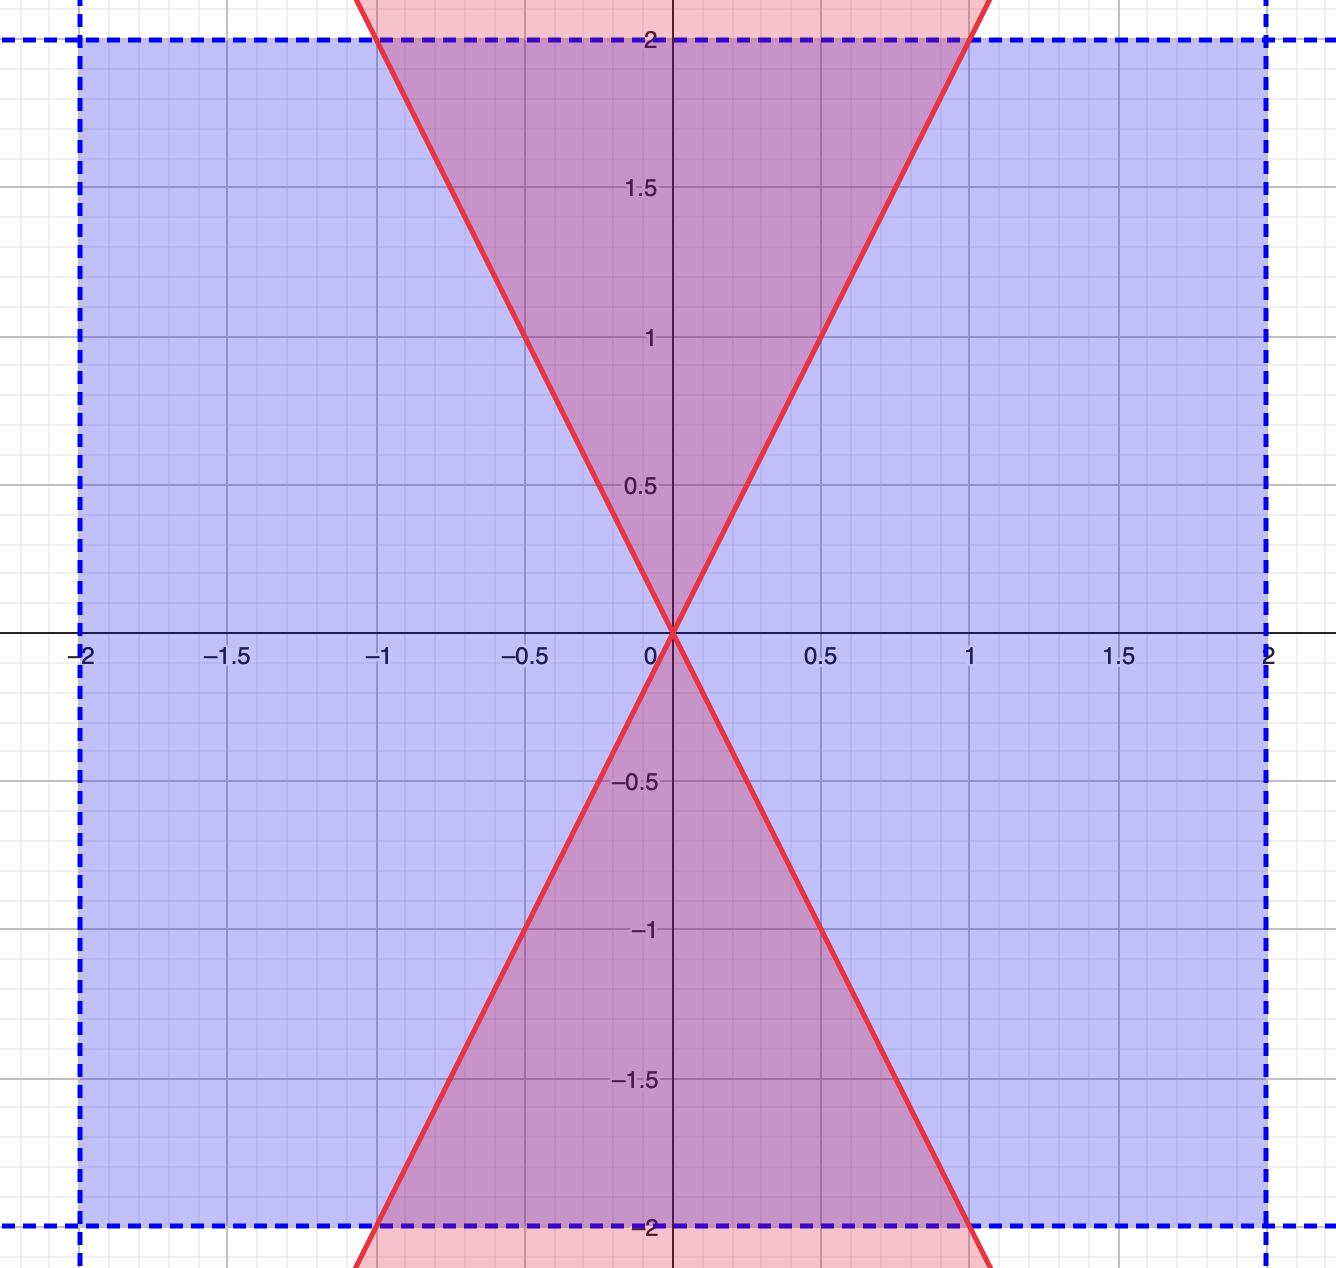
\includegraphics[width=0.5\textwidth]{test_1_problem_3.png}
    \caption{Квадрат $\Omega = [-2,2]\times[-2,2]$, зображений \textcolor{blue}{синім} кольором та область $(y-2x)(y+2x) \geq 0$, помічена \textcolor{red}{червоним} кольором.}
    \label{fig:problem_3_illustration}
\end{figure}

Також, з малюнку одразу видно, що обидві прямі перетинають верхню і нижню сторони квадрату $\Omega = [-2,2] \times [-2,2]$ (це звичайно можна було вивести і аналітично), тобто сторони, що лежать на прямих $y=\pm 2$. Тоді відповідні $x$ координати мають вигляд $x = \pm 1$. Отже, бачимо, що область $E$ -- це два рівнобічних трикутника з висотою $2$ (сторона квадрата) і базою $2$. Тому площа кожного з трикутників $\frac{2 \times 2}{2} = 2$, а отже сумарна площа $\lambda(E) = 2 \times 2 = 4$. Тому відповідь: $\text{Pr}[E] = \frac{4}{16} = \boxed{\frac{1}{4}}$.

\textbf{Відповідь.} Ймовірність дорівнює $1/4$.

\end{document}
